% 导言区
\documentclass[cct]{article}

\usepackage{ctex}

%标题、作者及日期
\title{插图}
\author{张三丰}
\date{\today}

%语法: \includegraphics[<选项>]{<文件名>}
%格式:	EPS,PDF,PNG,JPEG,BMP
\usepackage{graphicx}
\graphicspath{{figures/},{pics/}}%图片在当前目录下的figures目录下或者pics目录下
%设定图片浮动的宏包
\usepackage{float} 
%设定字图片的宏包
\usepackage{subfigure}
% 正文区(文稿区)
\begin{document}
	\maketitle
	\LaTeX{}中的插图:
	
	\begin{figure}[H] %H为当前位置,!htb为忽略美学标准,htbp为浮动图形
		\centering %图片居中
		%[]中填写的是可选参数,scale表示缩放因子,angle表示逆时针旋转角度,width表示宽度,height表示高度,不同的可选参数用逗号分隔
		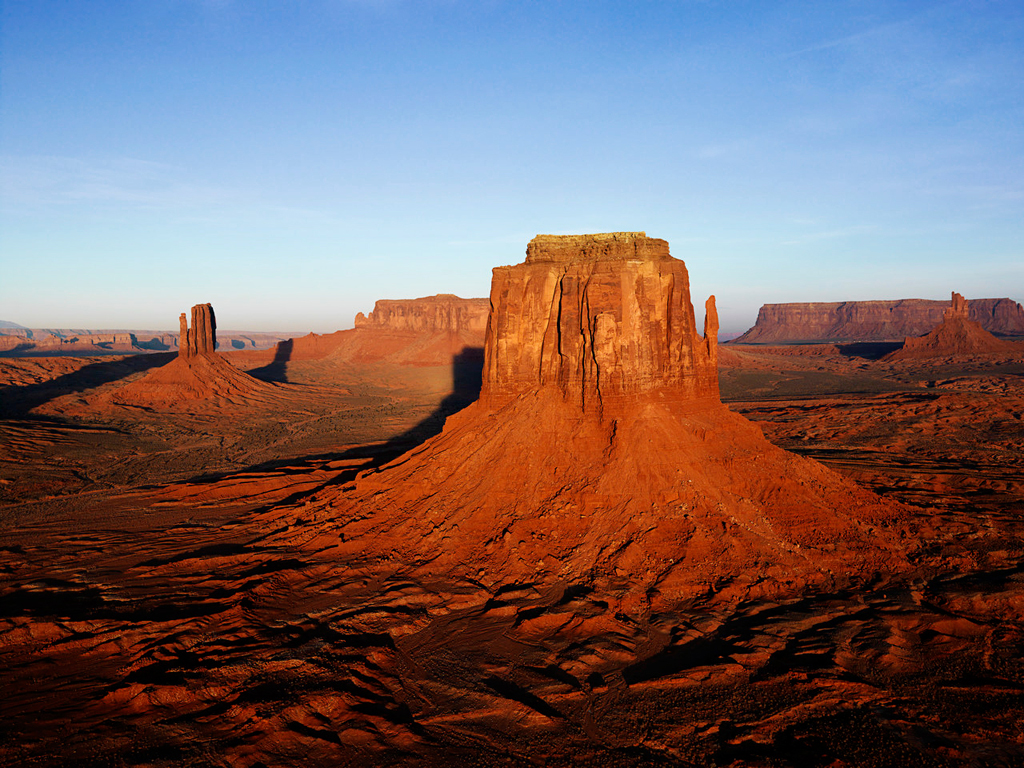
\includegraphics[scale=0.3,angle=30]{Desert.jpg}
		\caption{Main name 2} %最终文档中希望显示的图片标题
		\label{Fig.main2} %用于文内引用的标签
	\end{figure}
	Figure \ref{Fig.main} has two sub figures, fig. \ref{Fig.sub.1} is the travel demand of driving auto, and fig. \ref{Fig.sub.2} is the travel demand of park-and-ride.
	
	\begin{figure}[H]
		\centering  %图片全局居中
		\subfigure[name1]{
			\label{Fig.sub.1}
			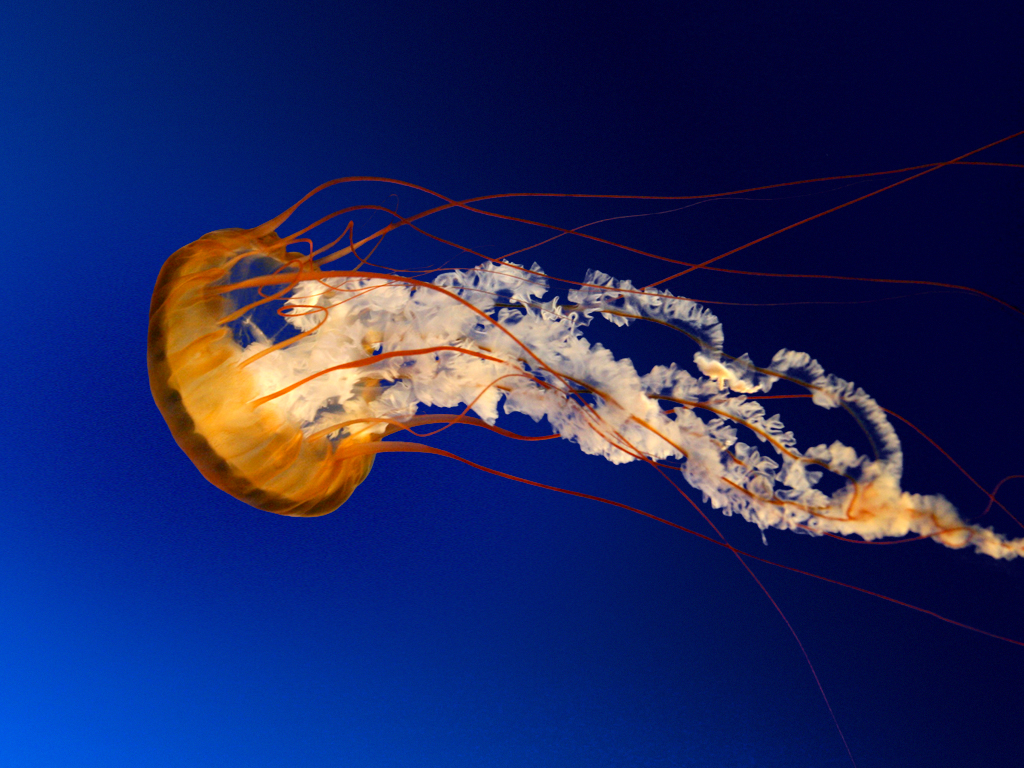
\includegraphics[width=0.45\textwidth]{Jellyfish}}
		\subfigure[name2]{
			\label{Fig.sub.2}
			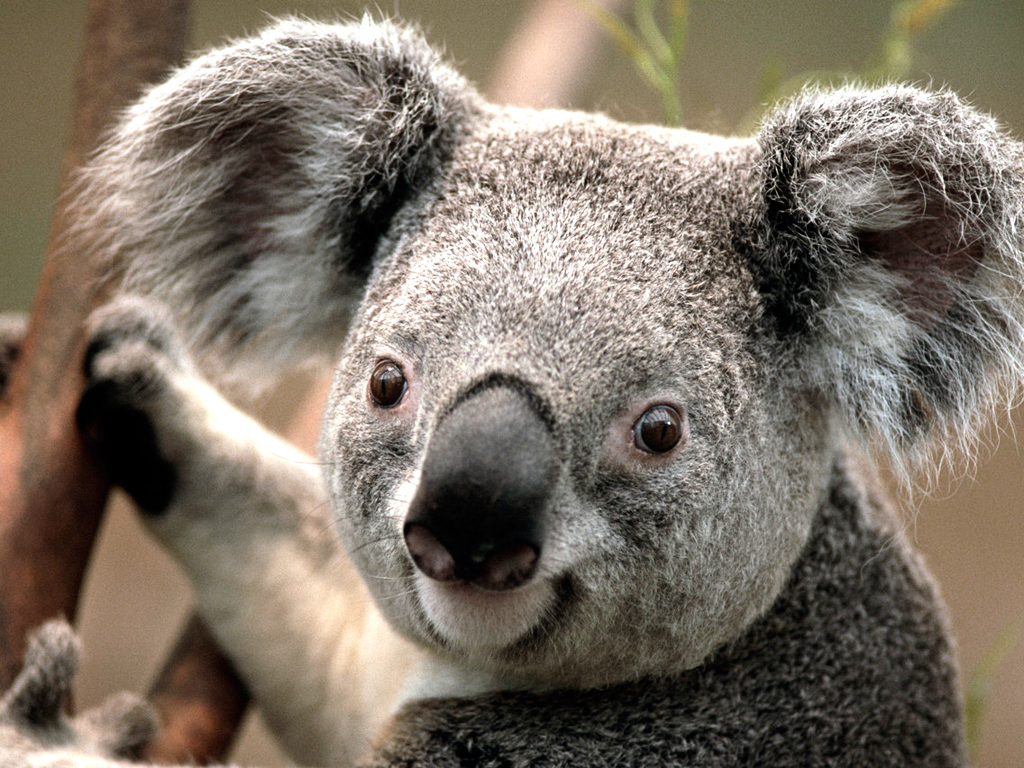
\includegraphics[width=0.45\textwidth]{Koala.jpg}}
		\caption{Main name}
		\label{Fig.main}
	\end{figure}
\end{document}